\documentclass[accentcolor=tud1a,colorbacktitle,inverttitle,landscape,german,presentation,t]{tudbeamer}
\usepackage{ngerman}
\usepackage{subcaption}
\usepackage{graphicx}

\begin{document}

\title{\"Ubung 5}
\subtitle{Visual Computing - Bilder}

\author[Johannes Beck, Christian Eilers, Robin Menzenbach, Martin Steinborn]{Johannes Beck, Christian Eilers, Robin Menzenbach, Martin Steinborn}

%\institute[IFP TUD]{Institut f"ur Festk"orperphysik, TU Darmstadt}

%\logo{\includegraphics{TUDbeamer-logo}}
% \logo{\color{tudtextaccent}\large IFP}

\date{\today}

\begin{titleframe}
\end{titleframe}

\section{Aufgabe 1}
	\begin{frame}
		\frametitle{Aufgabe 1: Tiefpass vs. Hochpass \\ a)}
		Bei dem ersten angeebenen Amplitudenspektrum handelt es sich um eienn Tiefpass-Filter. Dies ist is leicht daran zu erkennen, dass niedrige Frequenzen ungehindert passieren können, während hohe vollständig geblockt werden
		Das zweite Apmlitudenspektrum kann einem Hochpassfilter zugeordnet werden, da hier hohe Frequenzen ungestört passsieren, während niedrige gebockt werden.
	\end{frame}
	
	\begin{frame}
	\frametitle{Aufgabe 1: Tiefpass vs. Hochpass \\ b)}
	Ein Tiefpassfilter im Ortsraum kennzeichnet sich dadurch, dasss alle Koeffizienten positiv und normalisiert sind.Ebenfalls werden nur positive Werte produziert. Allerdings kann es zu Randeffekten kommen. %TODO Anwendungsbeispiel
	Bei einem Tiefpassfilter sind die Koeffizienten zwar ebenfalls normiert, können aber neben positiven auch negative Werte annehmen. Somit können nun auch negative Werte produziert werden. %TODO Anwendungsbeispiel
	
	\end{frame}

	\begin{frame}
	\frametitle{Aufgabe 1: Tiefpass vs. Hochpass \\ c)}
	%TODO 1c)
	
	\end{frame}
\section{Aufgabe 2}
	\begin{frame}
		\frametitle{Aufgabe 2: Pixeloperation und Filtermasken \\ a)}
			\label{2_a}
			Der unterschied zwischen einer Pixel-Operation und Filtermasken liegt darin, dass bei Pixel-Operationen das zu bearbeitende Pixel ohne Einfluss der Pixel in seiner Umgebung bearbeitet wird. SeineNachbarschaft spielt also keine Rolle.Bei Filtermasken ist dies exakt anders herum. hier werden Pixel in Abhängigket ihrer Nachbarshaft bearbeitet.Es spielt also nicht nur eine Rolle wie das entsprechende Pixel aussieht, sondern auch wie es um es herum aussieht.
	\end{frame}

	\begin{frame}
		\frametitle{Aufgabe 2: Pixeloperation und Filtermasken \\ b)}
		%TODO Hab ich gegoogelt, bin mir aber net sicher
		Das Problem von Filtermasken bei der Verwendung am Rande eines Bildes besteht darin, dass sie wie in \ref{2_a} beschrieben eben nicht nur auf das zu bearbeitende Pixel zugreifen um es  zu verändern, sondern auch um die Pixel in der direkten Nachbarschaft. Dies gechieht in alle Richtungen gleichermaßen und somit entsteht das Problem, dass am Rand eine Richtung eben keine benachbarten Pixel mehr hat und somit die Filttermaske auf nicht existierende Pixel zugreifen müsste. Zwei mögliche Lösungen dieses Problems sind zum Beispiel am Rand keine Filter anzuwenden. Dadurch gäbe es keine zugriffe außerhalb der Daten und das Problem wäre gelöst. Als zweite Option könnte man den letzten verfügbaren Wert benutzen, um unzulässige Zugriffe zu vermeiden. 
	\end{frame}
	
	\begin{frame}
		\frametitle{Aufgabe 2: Pixeloperation und Filtermasken \\ c)}
		%TODO soll man hier rand und filter getrennt angeben und passst das mit der randmethode?
	
		Die Anwendung eines 3x3 Mittelwert-Filters auf das gegebene Graustufenbild liefert
		\begin{align*}
		\begin{bmatrix}
		230 & 15 & 220 & 158 & 100 \\
		156 & 131 & 115 & 111.444 & 19\\
		7 & 111.444 & 115.333 & 98.333 & 103\\
		88 & 103.222 & 121.778 & 106.333 & 73\\
		142 &234 & 67 & 186 & 28
		\end{bmatrix}
		\end{align*}
		als Ergebnis. Zur Randbehandlung wude die Methode gewählt, am rand keinen Flter anzuwenden.
	\end{frame}

\section{Aufgabe 3}
	\begin{frame}
		\frametitle{Aufgabe 3: Digitale Kamera \\ a)}
		%TODO 3a)
	\end{frame}
	
	\begin{frame}
		\frametitle{Aufgabe 3: Digitale Kamera \\ b)}
		%TODO 3b)
	\end{frame}
	
	\begin{frame}
		\frametitle{Aufgabe 3: Digitale Kamera \\ c)}
		%TODO 3c)
	\end{frame}
\section{Aufgabe 4}
	\begin{frame}[t]
		\frametitle{Aufgabe 4: Histogrammausgleich}
		\begin{figure}
		\centering
		\begin{minipage}[c]{.2\textwidth}
			\centering
			$\begin{bmatrix}
			6& 48& 94& 33& 7\\
			12& 36& 26& 71& 91\\
			29& 17& 34& 45& 67\\
			34& 55& 74& 1& 41\\
			87& 14& 28& 61& 32
			\end{bmatrix}$
		\end{minipage}
		\begin{minipage}[c]{.2\textwidth}
			\centering
			$\huge \Rightarrow$
		\end{minipage}
		\begin{minipage}[c]{.3\textwidth}
			\centering
			$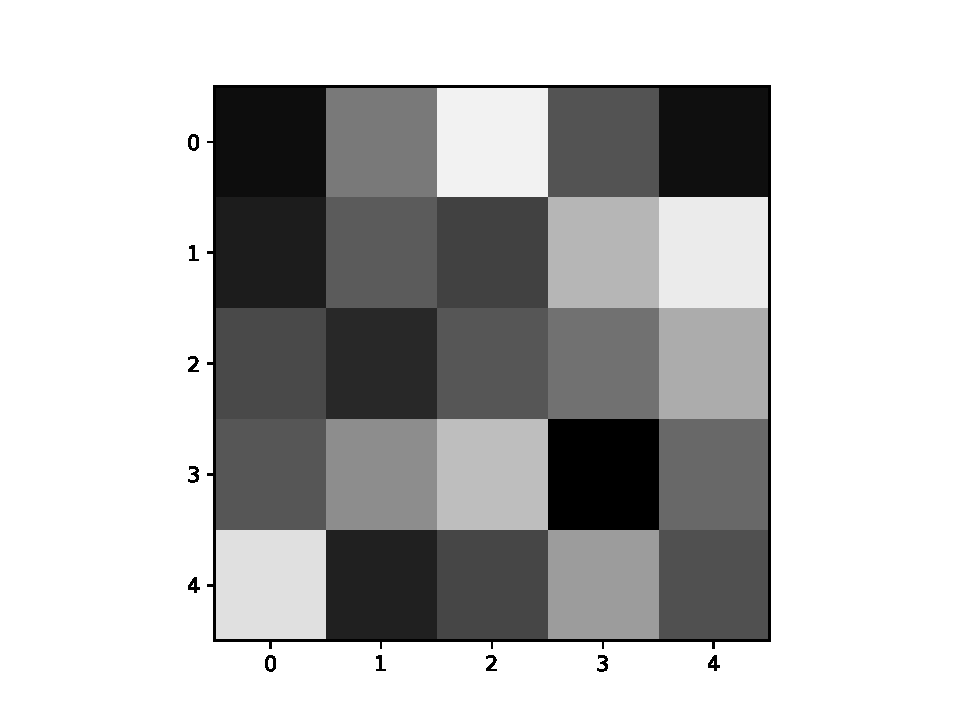
\includegraphics[width=\textwidth]{fig/image.pdf}$
		\end{minipage}

		
		\end{figure}

		
	\end{frame}
	\begin{frame}[t]
		\frametitle{Aufgabe 4: Histogrammausgleich}
		\begin{figure}	
			\centering
			\begin{subfigure}[t]{.45\textwidth}
				\centering
				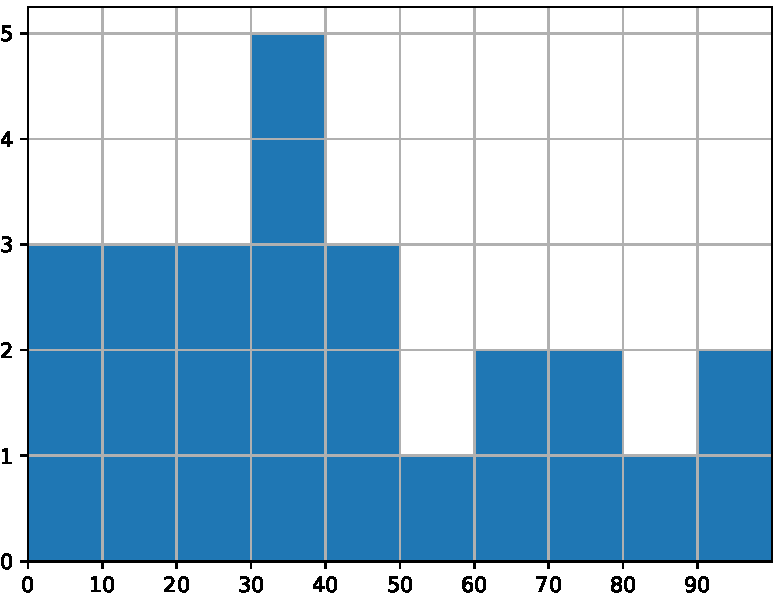
\includegraphics[width=\textwidth]{fig/histogram.pdf}
				\caption{Histogramm}\label{fig:1a}		
			\end{subfigure}
			\quad
			\begin{subfigure}[t]{.45\textwidth}
				\centering
				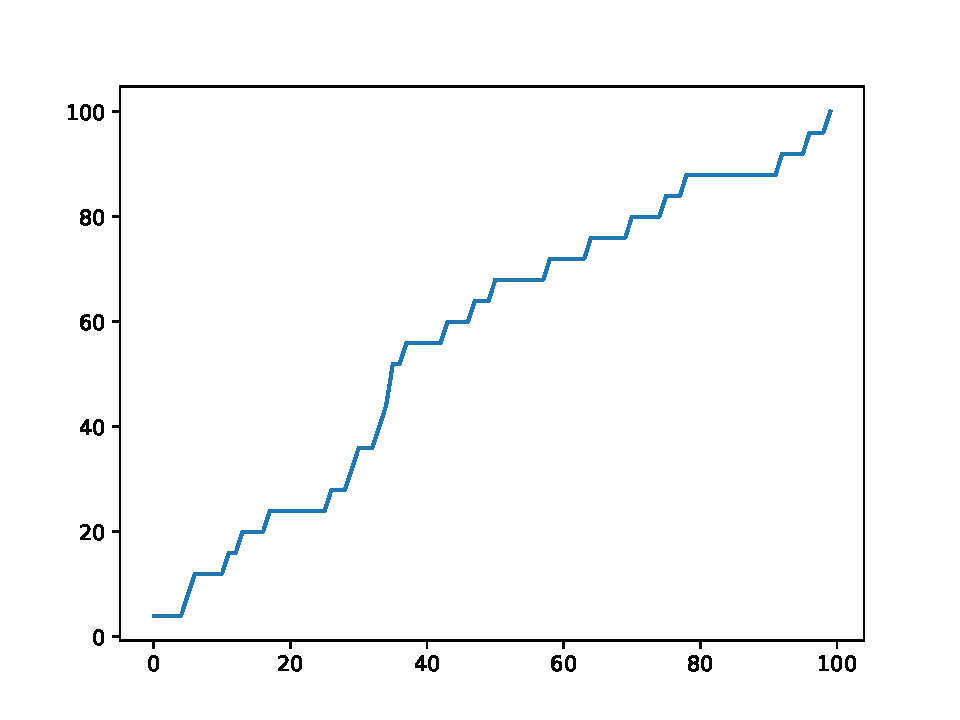
\includegraphics[width=\textwidth]{fig/s-curve.pdf}
				\caption{S-Kurve}\label{fig:1b}
			\end{subfigure}
			\caption{Plots}\label{fig:1}
		\end{figure}
	\end{frame}
\end{document}